\documentclass{beamer}
\usepackage[utf8]{inputenc}

\usetheme{Madrid}
\usecolortheme{default}
\usepackage{amsmath}
\usepackage{amssymb,amsfonts,amsthm}
\usepackage{txfonts}
\usepackage{tkz-euclide}
\usepackage{listings}
\usepackage{adjustbox}
\usepackage{array}
\usepackage{tabularx}
\usepackage{gvv}
\usepackage{lmodern}
\usepackage{circuitikz}
\usepackage{tikz}
\usepackage{graphicx}

\setbeamertemplate{page number in head/foot}[totalframenumber]

\usepackage{tcolorbox}
\tcbuselibrary{minted,breakable,xparse,skins}



\definecolor{bg}{gray}{0.95}
\DeclareTCBListing{mintedbox}{O{}m!O{}}{%
  breakable=true,
  listing engine=minted,
  listing only,
  minted language=#2,
  minted style=default,
  minted options={%
    linenos,
    gobble=0,
    breaklines=true,
    breakafter=,,
    fontsize=\small,
    numbersep=8pt,
    #1},
  boxsep=0pt,
  left skip=0pt,
  right skip=0pt,
  left=25pt,
  right=0pt,
  top=3pt,
  bottom=3pt,
  arc=5pt,
  leftrule=0pt,
  rightrule=0pt,
  bottomrule=2pt,
  toprule=2pt,
  colback=bg,
  colframe=orange!70,
  enhanced,
  overlay={%
    \begin{tcbclipinterior}
    \fill[orange!20!white] (frame.south west) rectangle ([xshift=20pt]frame.north west);
    \end{tcbclipinterior}},
  #3,
}
\lstset{
    language=C,
    basicstyle=\ttfamily\small,
    keywordstyle=\color{blue},
    stringstyle=\color{orange},
    commentstyle=\color{green!60!black},
    numbers=left,
    numberstyle=\tiny\color{gray},
    breaklines=true,
    showstringspaces=false,
}
\title{2.0.25}
\date{26th March, 2026}
\author{Vishwambhar - EE25BTECH11025}

\begin{document}

\frame{\titlepage}
\begin{frame}{Question}
If $log_e(y)=-xlog_e(y)$, then the maximum value of $y$ is
\begin{enumerate}
    \item $e$
    \item $e^{x^2}$
    \item $e^{e^{-1}}$
    \item $e^x$
\end{enumerate}
\end{frame}

\begin{frame}{Goal}
We want to maximize,
\begin{align}
    f\brak{x} = -xlog\brak{x}
\end{align}
Constraint $x>0$
\end{frame}

\begin{frame}{Gradient}
\begin{align}
\nabla f\brak{x}=-\brak{logx+1}
\end{align}
\begin{enumerate}
    \item If $\nabla f\brak{x}>0$  function increasing
    \item If $\nabla f\brak{x}<0$  function decreasing
    \item If $\nabla f\brak{x}=0$  possible max/min
\end{enumerate}
solving for option 3 we get,
\begin{align}
x=e^{-1}
\end{align}
\end{frame}

\begin{frame}{Hessian}
\begin{align}
\nabla^2f\brak{x}=\frac{-1}{x}
\end{align}
If Hessian > 0 curve opens upward
If Hessian <0 curve opens downward
Here:
\begin{align}
    \frac{-1}{x}<0 \forall x>0
\end{align}
\end{frame}

\begin{frame}{Conclusion}
Since the curve is concave the maximum will occur at a stationery point which is $x=\frac{1}{e}$.
\end{frame}

\begin{frame}{Plot-y}
    \begin{figure}
        \centering
        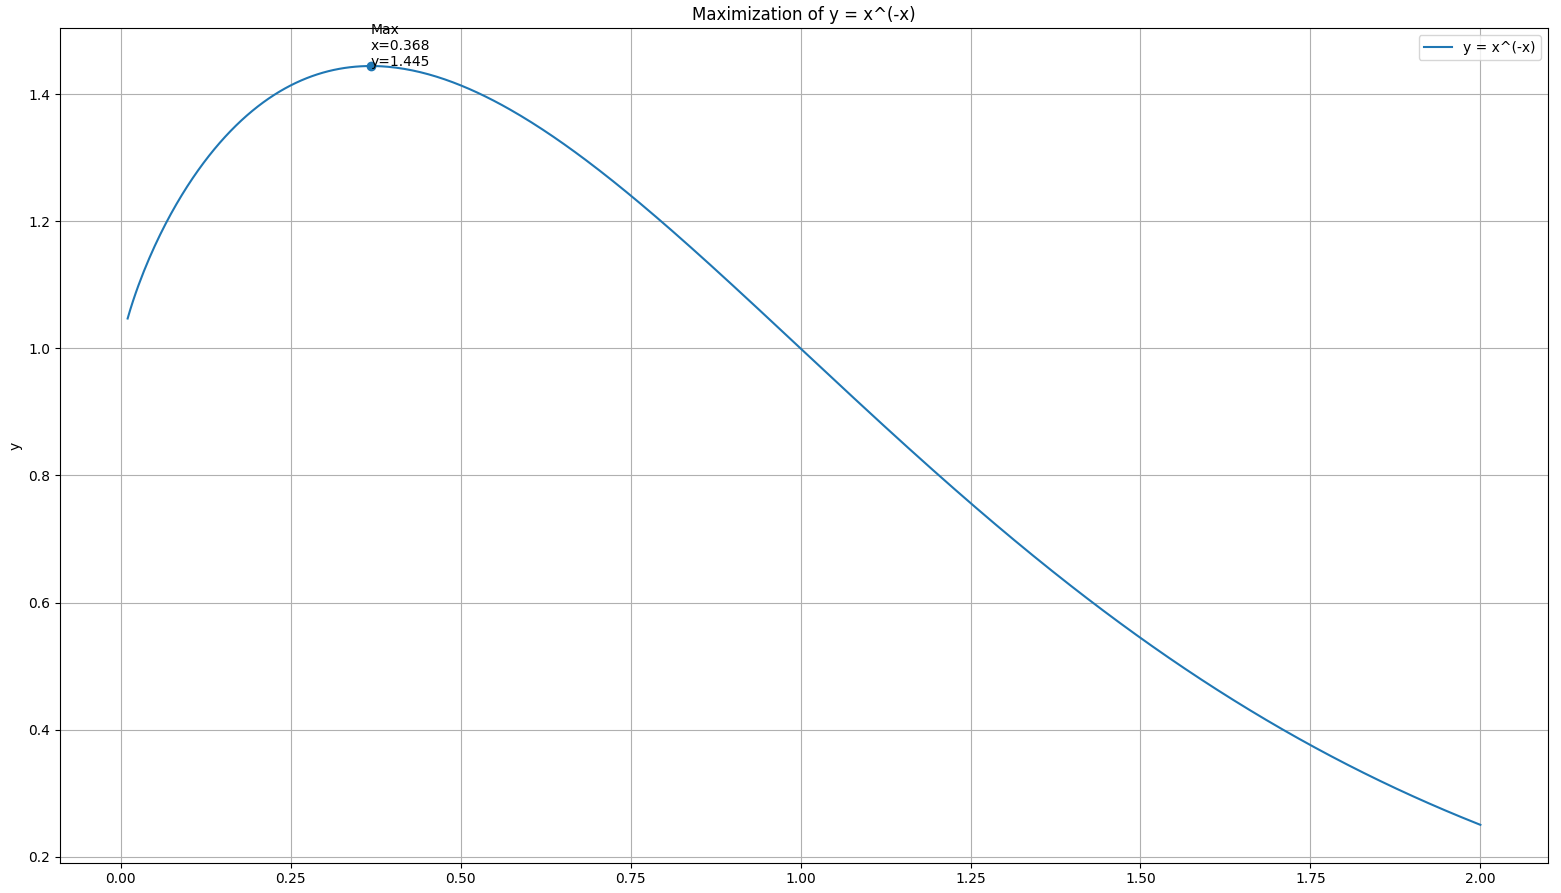
\includegraphics[width=1\columnwidth]{figs/plot.png}
        \label{fig:fig}
    \end{figure}
\end{frame}

\begin{frame}[fragile]
    \frametitle{Python Code}
    \begin{lstlisting}
import cvxpy as cp
import numpy as np
import matplotlib.pyplot as plt

x = cp.Variable(pos=True)
objective = cp.Maximize(cp.entr(x))
constraints = [x >= 1e-6]

prob = cp.Problem(objective, constraints)
prob.solve()

x_opt = x.value
y_opt = np.exp(-x_opt * np.log(x_opt))

x_vals = np.linspace(0.01, 2, 500)
y_vals = np.exp(-x_vals * np.log(x_vals))
    \end{lstlisting}
\end{frame}

\begin{frame}[fragile]
    \frametitle{Python Code}
    \begin{lstlisting}
plt.figure()
plt.plot(x_vals, y_vals, label="y = x^(-x)")
plt.scatter(x_opt, y_opt)
plt.text(x_opt, y_opt,
         f"Max\nx={x_opt:.3f}\ny={y_opt:.3f}")
plt.xlabel("x")
plt.ylabel("y")
plt.title("Maximization of y = x^(-x)")
plt.legend()
plt.grid()

plt.show()
    \end{lstlisting}
\end{frame}
\end{document}